\documentclass{standalone}


\usepackage{tikz}
\usepackage{pgfplots}
\usetikzlibrary{calc}
\pgfplotsset{compat=1.15}
\usetikzlibrary{shapes,arrows.meta}
\begin{document}


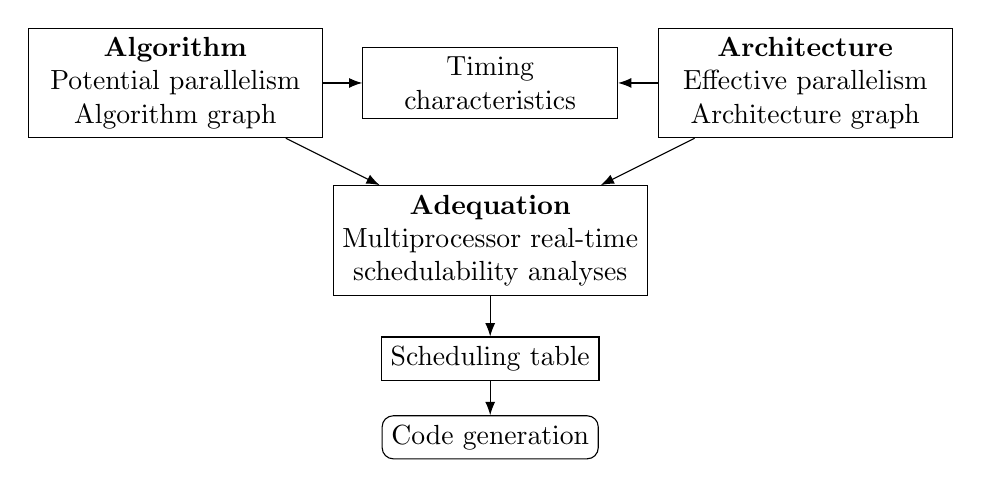
\begin{tikzpicture}[>=Latex,node distance=2cm]
\node[rectangle,draw,text width=3cm,align=center,minimum width=2cm] (char) {Timing\\characteristics};
\node[rectangle,draw,left of = char,text width=3.5cm,xshift=-2cm,align=center] (algo) {\textbf{Algorithm}\\Potential parallelism\\Algorithm graph};
\node[rectangle,draw,right of = char,text width=3.5cm,xshift=2cm,align=center] (arch) {\textbf{Architecture}\\Effective parallelism\\Architecture graph};
\node[rectangle,draw,below of = char,align=center] (adeq) {\textbf{Adequation}\\Multiprocessor real-time\\schedulability analyses};
\node[rectangle,draw,below of = adeq,align=center,yshift=.5cm] (sched) {Scheduling table};
\node[rectangle,draw,below of = sched,rounded corners,align=center,yshift=1cm] (code) {Code generation};

\draw [->] (algo) -- (char);
\draw [->] (arch) -- (char);
\draw [->] (algo) -- (adeq);
\draw [->] (arch) -- (adeq);
\draw [->] (adeq) -- (sched);
\draw [->] (sched) -- (code);


\end{tikzpicture}

\end{document}